\documentclass[12pt, varwidth, border=5mm]{standalone}
\usepackage{tikz}
\usepackage{amsmath}
% Underlining package
\usepackage{ulem}
\usetikzlibrary{angles,quotes}
\usetikzlibrary{intersections}
\usetikzlibrary{arrows.meta}
\usetikzlibrary{calc}
% \usepackage[a4paper, portrait, margin=1cm]{geometry}


\begin{document}
\section*{ }
    
$\text{e} = \text{70}^\circ$
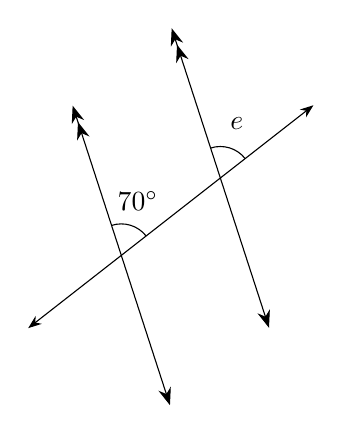
\begin{tikzpicture}[scale=1.0, baseline=(current bounding box.north)]
  \begin{scope}[rotate=38]
    % Draw the first line
    \draw[<->>, >={Stealth[scale=1.3]}, name path=P1] (0, 0) -- (1.3680805733026753, 3.7587704831436333);
    % Draw the second line with the calculated offsets
    \draw[<->>, >={Stealth[scale=1.3]}, name path=P2] (1.5962666587138683, 0) -- (2.964347232016544, 3.7587704831436333);
    % Draw the transversal through the middle of the parallel lines
    \draw[<->, >=Stealth, name path=P3] (-0.8159597133486622, 1.8793852415718166) -- (3.780306945365206, 1.8793852415718166);
    \path [name intersections={of=P1 and P3,by=A}];
    \path [name intersections={of=P2 and P3,by=B}];
    % Draw the angle
    \coordinate (p1s) at (0, 0);
    \coordinate (p1e) at (1.3680805733026753, 3.7587704831436333);
    \coordinate (p2s) at (1.5962666587138683, 0);
    \coordinate (p2e) at (2.964347232016544, 3.7587704831436333);
    \coordinate (ts) at (-0.8159597133486622, 1.8793852415718166);
    \coordinate (te) at (3.780306945365206, 1.8793852415718166);
    \draw pic["$e$", draw=black, -, angle eccentricity=1.8, angle radius=0.4cm] {angle=te--B--p2e};
\draw pic["$70^\circ$", draw=black, -, angle eccentricity=1.8, angle radius=0.4cm] {angle=te--A--p1e};

  \end{scope}
\end{tikzpicture}

\end{document}
